\documentclass[tikz,border=3pt]{standalone}
\usetikzlibrary{arrows.meta,decorations.pathmorphing}
\begin{document}
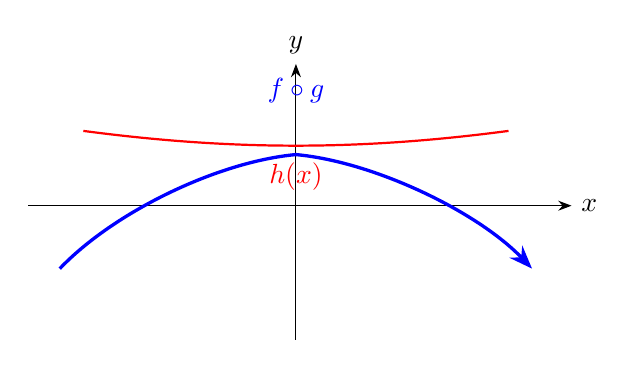
\begin{tikzpicture}[x=1cm,y=1cm,>=Stealth]
  \draw[->] (-3.4,0) -- (3.5,0) node[right] {$x$};
  \draw[->] (0,-1.7) -- (0,1.8) node[above] {$y$};
  \draw[blue,very thick,-Stealth,decorate,
    decoration={bent,aspect=.28,amplitude=3.5mm}]
    (-3,-.8) -- (0,.65) -- (3,-.8);
  \draw[red,thick,decorate,
    decoration={bent,aspect=.35,amplitude=-2.5mm}]
    (-2.7,.95) -- (2.7,.95);
  \node[blue,above] at (0,1.18) {$f\circ g$};
  \node[red,below] at (0,.67) {$h(x)$};
\end{tikzpicture}
\end{document}
